\documentclass[a4paper]{article}
\usepackage[utf8]{inputenc}
\usepackage[a4paper, total={6in, 8in}]{geometry}
\usepackage{amsmath}
\usepackage{graphicx}
\usepackage{setspace}
\usepackage{biblatex}
\addbibresource{Mendeley.bib}

\title{Graduate Research Plan Statement}
\author{Matthew Moreno}

\begin{document}
\maketitle

\doublespacing

\section{Motivation} \label{sec:motivation}
The exquisite matching of form to function in biological systems has long been admired by engineers. This admiration has given rise to the field of biomimicry, where design elements generated by nature are extracted to be employed in technological applications. Examples of biomimicry include legged locomotion in robotics that provides both efficiency and maneuverability \cite{Grimes2012THE}, nanotextures mimicking shark skin on boats that discourage barnacles growth while simultaneously decreasing water drag on the vessel \cite{Stenzel2011Drag-reducingShipping}, and tire treads inspired by the wet-adhesive properties of tree frog toe pads \cite{Persson2007WetTires}. In the field of computer science, great successes in solving otherwise intractable problems have been achieved by abstracting a high-level biological information-processing scheme: neural networks. Through this approach, engineers have designed systems that recognize different types of objects in images \cite{KrizhevskyImageNetNetworks}, convincingly beat the top-ranked human player at the notoriously high branching-factor board game Go \cite{Silver2016MasteringSearch}, and--although traditionally thought of as quintessentially human and inaccessible to an algorithmic approach--render images in distinct artistic styles learned by example (Figure \ref{fig:nn_art_styles}) \cite{Gatys2015AStyle}.

\begin{figure}
\centering
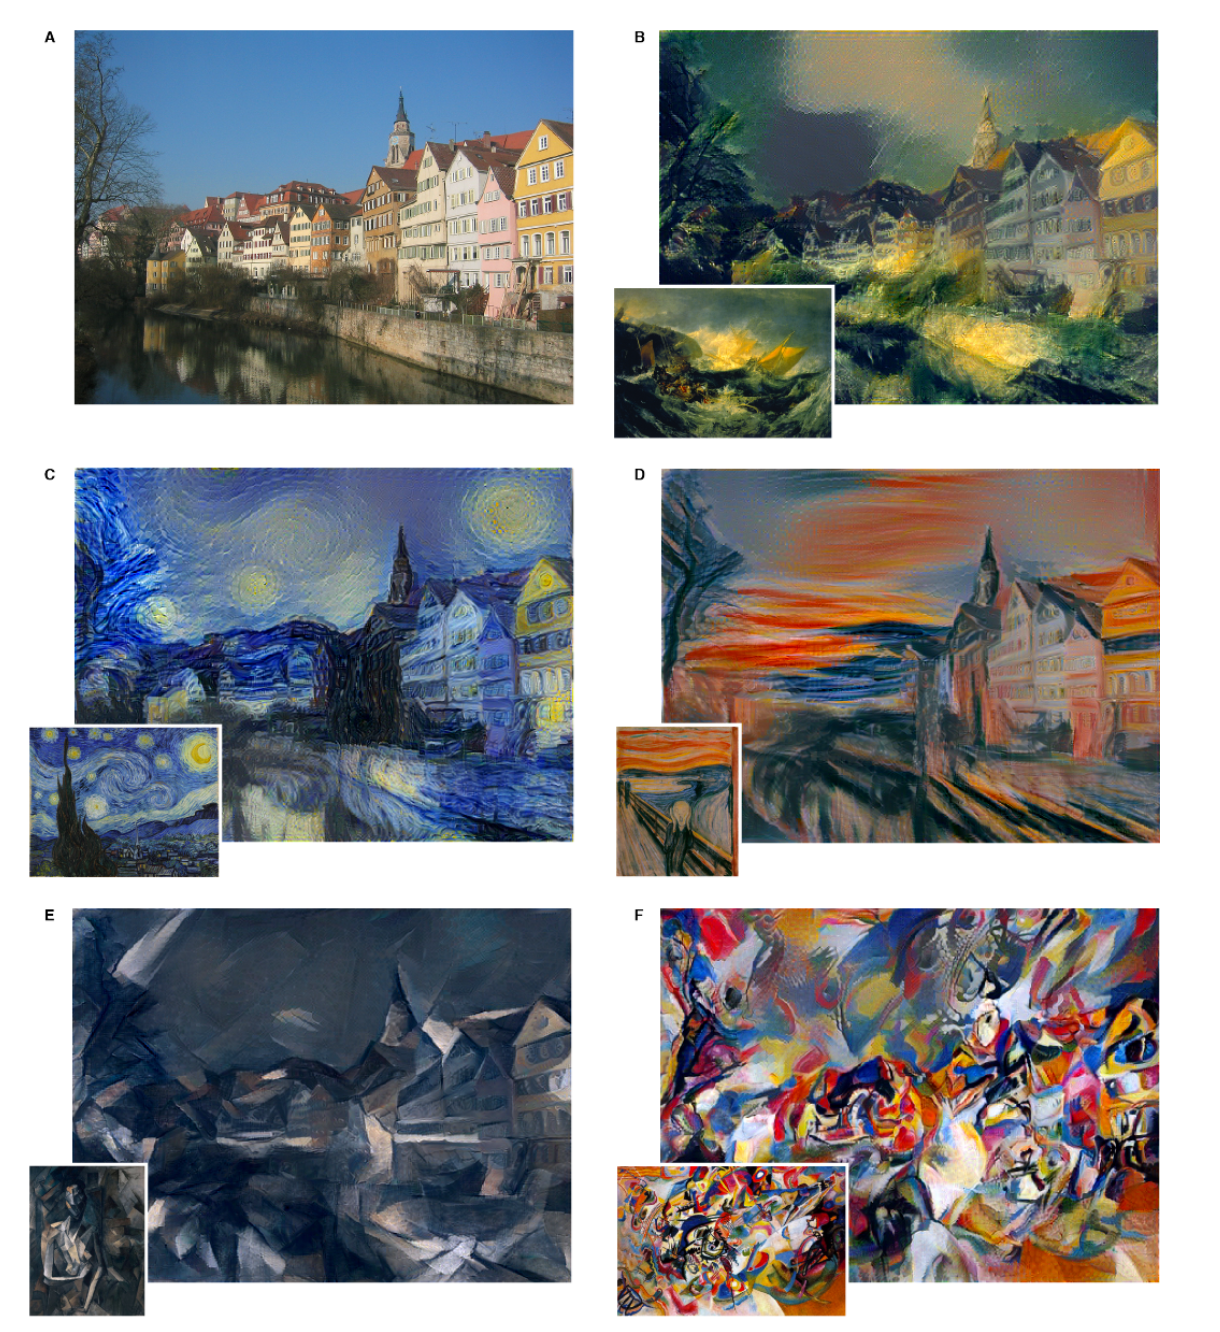
\includegraphics[width=0.5\textwidth]{nn_art_styles.png}
\caption{\label{fig:nn_art_styles} Application of various artistic styles to a content-image achieved through deep neural networks \cite{Gatys2015AStyle}} 
\end{figure}
Although the functionality exhibited by biological systems, the high fitness of individual phenotypes is spectacular, another marvel of biology lurks just behind the parade of sundry phenotypes well-suited to their respective environments: the genotype-phenotype mapping. Although this mapping might be naively dismissed as a mere implementation detail, it contributes to a number of properties essential to the evolutionary process. Among others, these include modularity, neutrality, robustness, weak linkage, and degeneracy \cite{Richter2015EvolvabilitySurvey, DowningIntelligenceSystems}. Although the importance of the genotype-phenotype mapping is non-obvious when considering the phenotypes of individuals in isolation, its importance becomes clear when viewing them in the larger evolutionary context of life: the genotype-phenotype mapping made the phenotypic forms observed in nature accessible to the evolutionary process in the first place. The evolutionary search would be stymied just traversing the raw phenotypic space. Take, for example, the repetition of structure at the very root of the cellular nature of life, the symmetries of biological forms, or the surprising  reapplications of existing mechanisms (such as ion flows in neural signaling), all of which would almost certainly be inaccessible in a phenotype-based search space. The genotype-phenotype mapping reorganizes the evolutionary search space, placing relative distant phenotypes in close evolutionary proximity. Consider Figure \ref{fig:arabidopsis_mutants}, which compares Wild Type \textit{Arabidopsis thaliana} with five mutant strains. These individuals are clustered together in the genotypic space of \textit{Arabidopsis thaliana}. Although the genotypic distance between these phenotypes is small, a relatively broad range of phenotypes is represented. While none of these the mutations would seem to confer selective advantage, they are representative of the rich diversity of form that is accessible to evolutionary search, allowing rapid adaptation to environmental changes or novel adaptation to the existing environment. Figure \ref{fig:arabidopsis_mutants} illustrates, in particular, the modularity of the system under genotype-phenotype mapping; the mutant strains exhibit significant variability in overall composition of the individual while preserving the general character of existing components. Although not illustrated in Figure \ref{fig:arabidopsis_mutants}, the local genotypic neighborhood also maps to a great number of phenotypes indistinguishable from Wild Type individuals, specimens that differ by more calibration-like adjustments to various properties of form, as well as--doubtlessly--fundamentally defective phenotypes. Further, the phenotype (for the most part) is known to exhibit stability under ordinary operations on the genetic space, such as recombination via crossover.

This project will investigate how genotype-phenotype mapping induces evolvability--making high-fitness individuals accessible via evolutionary search--in the context of Evolving Artificial Neural Networks (EANN). It is hoped that, although perhaps not through this individual piece of work, this line of inquiry will ultimately contribute to the development of more capable and versatile artificial intelligence systems.

\begin{figure}
\centering
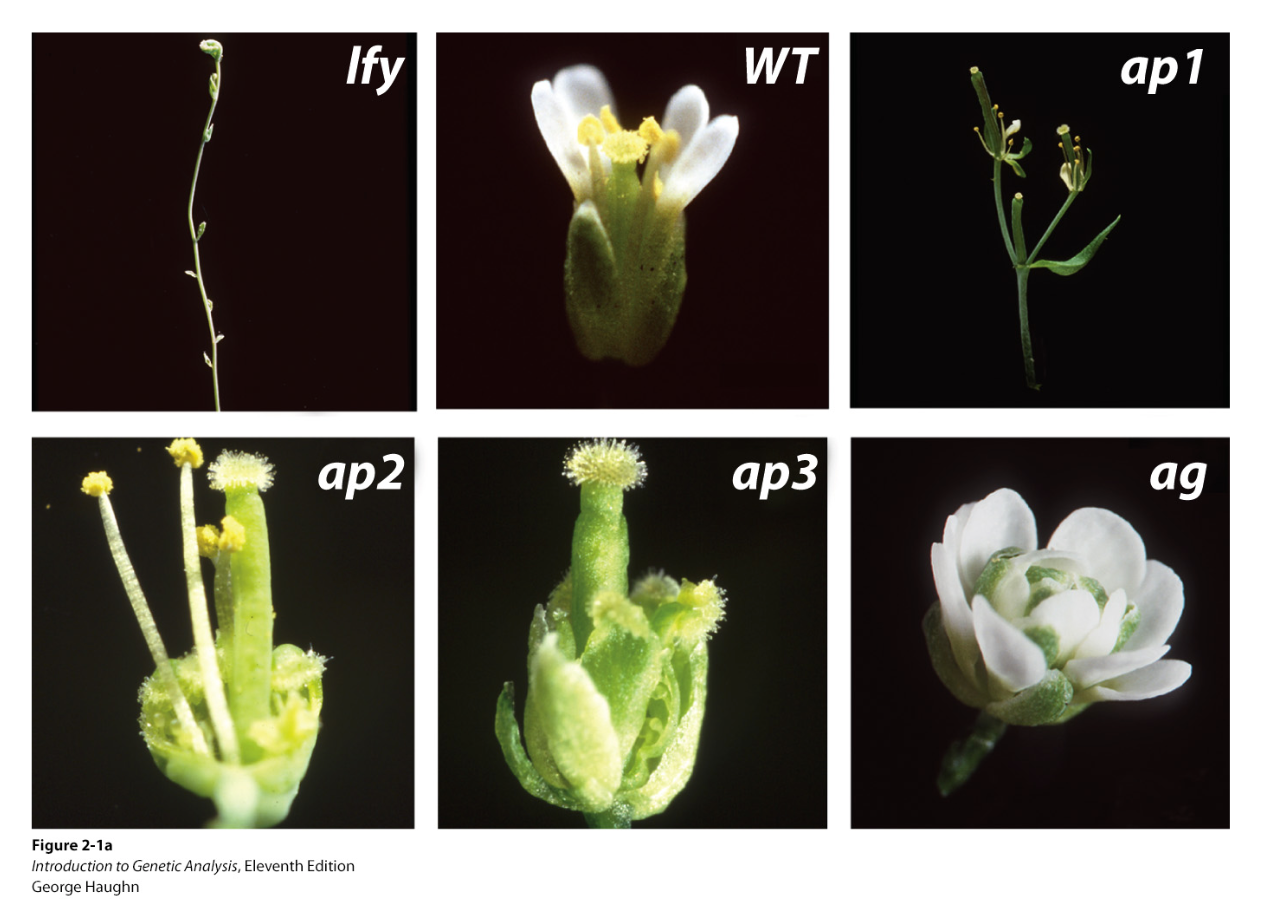
\includegraphics[width=0.6\textwidth]{arabidopsis_mutations.png}
\caption{\label{fig:arabidopsis_mutants}Wild-type and mutant strains of \textit{Arabidopsis thaliana} \cite{Griffiths2015IntroductionAnalysis}} 
\end{figure}

\section{Background}
\subsection{Evolutionary Algorithms}
At the genesis of modern computing, the 1950s, researchers began to apply advancing computational capabilities to investigate and test models of biological evolution. Very quickly they realized the potential of virtual evolution to achieve other ends, setting into motion a line of research that has since blossomed into the field of evolutionary algorithms (EA) design. These algorithms, which use mechanics inspired by biological evolution to evolve novel solutions to a wide array of problems, share a generally consistent basic methodology. The process begins with a population of randomly generated solutions. In a generation-based loop, an elite subset of the population is selected for their fitness (their quality as a solution), subjected to random changes, and recombined with each other to form the next generation. The cycle repeats for as many iterations as desired, and fitness tends to increase with each iteration. Figure \ref{fig:working_principle} provides a graphical overview of this process.
\begin{figure}
\centering
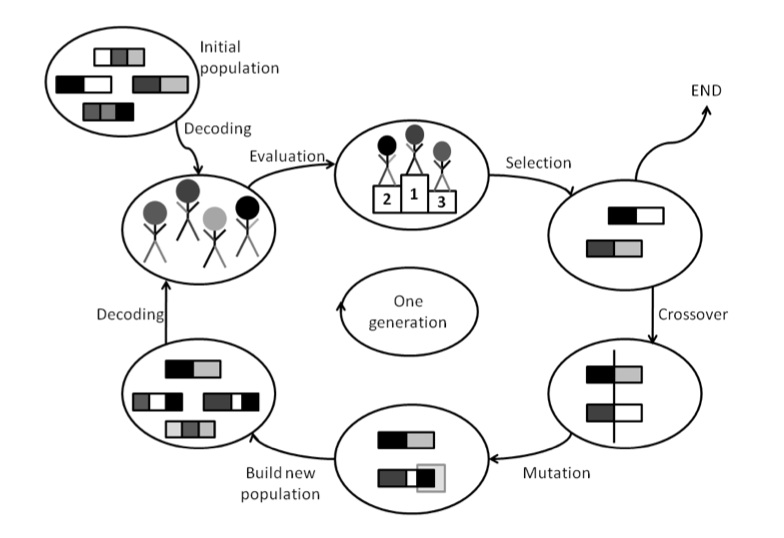
\includegraphics[width=0.5\textwidth]{working_principle_of_EA.jpg}
\caption{\label{fig:working_principle} The working principle of evolutionary algorithms \cite{Prothmann2009EvolutionaryOptimisation}} 
\end{figure}


Researchers and engineers have widely demonstrated the ability of EA to attack labor-intensive optimization problems and to discover novel solutions beyond the reach of human ingenuity. The intervening half century of EA research has seen diversification of the general evolutionary search process described above and branching of the contents and format of candidate solutions. Solutions can be a set of real values, such as the component dimensions of a satellite truss optimized through EA by NASA to minimize vibration resistance. Solutions can also be represented as branched connections between operations and values, colloquially known as a ‘tree.’ This type of EA is known as genetic programming (GP). Essentially, candidate solutions in traditional GP are mathematical expressions formatted for flexibility in recombination and manageability of expression in code. \cite{Poli2008AProgramming}. A distinction can also be drawn between mutation-based approaches such as evolution strategies or evolutionary programming and crossover-based approaches, which rely on distinct theory based around the concept of schemata, the collections of fixed points on chromosomal bitstrings that, as a unit, confer fitness to an individual \cite{2006RepresentationsAlgorithms}. In practice, however, a combination of crossover and mutation, to generate background noise to the process, is typically favored, such as the standard simple genetic algorithm (GA).

\subsection{Neural Networks}

Neural networks, as mentioned in Section \ref{sec:motivation}, have rapidly cemented themselves as a cornerstone of modern computer science. These systems are loosely modeled on the distributed neural architecture of the brain. At the most basic level, neural networks can be described as a chain of weighted and re-scaled sums. These networks are traditionally organized into distinct, ordered layers of nodes, with each layer determining its values based on those of the previous layer and the first and last representing input and output, respectively, of the network. This scheme is called ``feed-forward'' because information flows from one layer to the next and out of the system, and is not retained in the system through cyclic topologies. A prototypical feed-forward network is illustrated in Figure \ref{fig:feed_forward}. Networks are typically initiated with random or uniform initial connectivity weightings, which are refined through an iterative trial-and-error-driven process known as training where the network is adjusted towards exhibiting a desired behavior. Recent advances in the field have been made by employing back-propagation with deep neural networks, that is neural networks with many hidden layers between the input and output layers. While this method is both powerful and computationally tractable, it has significant limitations  including the necessity of instantaneous feedback during the training process (each training input must be coupled with a known, desired output), poor ability to train networks with recurrence (i.e. networks with memory), the possibility of getting stuck at local maxima, and lack of network adaptability post-training \cite[pg 312, 364]{DowningIntelligenceSystems}. 
\begin{figure}
\centering
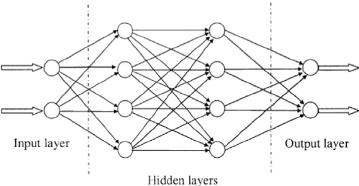
\includegraphics[width=0.6\textwidth]{Fig-1-Schematic-diagram-of-a-multilayer-feed-forward-neural-network-3.png}
\caption{\label{fig:feed_forward} An illustration of a feed-forward neural network with two hidden layers \cite{Griffiths2015IntroductionAnalysis}} 
\end{figure}


\section{Topic}

This project will focus on Evolving Artificial Neural Networks (EANN), a widely-explored alternative to back-propagation paradigm of network training \cite{DowningIntelligenceSystems}. Although more lax in the required frequency of feedback provision during the training process and more friendly to training with recurrent structures, this approach can be stymied by its own set of challenges. In particular, designing these systems to be highly evolvable--making them compatible with the evolutionary process by avoiding excessive fatal mutations and premature dead-end local maxima in the search space, for instaance--is a non-trivial task (especially for large networks). It is thought that moving beyond direct encodings, genotypic encodings where each topological connection and weight is explicitly specified, to adaptive, implicit, or generative genotype-phenotype mappings might address these issues. Promising research has been conducted in this vein. A prime example is the Genetic Regulatory Network (GRN) scheme of Reisinger and Miikkulainen, which they found yielded a more compact representation, more adaptive variation, and more robustness to mutation compared to the direct encoding (as well as alternate encodings) \cite{ReisingerAcquiringRepresentations}. This GRN scheme is just one of a number of genotype-phenotype mappings have been explored, such as Neuroevolution of Augmenting Topologies (NEAT), cellular encoding (CE), and encodings based on context-free grammars \cite{DowningIntelligenceSystems}.


\section{Project Objectives}
The objective of this project is to survey the existing approaches to genotype-phenotype mappings for EANN in order to understand their algorithmic implementation as well as their design principles. These principles will be synthesized with design principles gleaned from evolutionary biology and neuroscience to develop a broad conceptual framework describing the problem of genotype-phenotype mapping in the context of EANN. This project will culminate in the design of experiments to investigate how the absolute performance (measured in average number of generational iterations to convergence and best individual fitness attained) and various evolvability metrics (such as robustness, neutrality, acquired evolvability, etc. \cite{Richter2015EvolvabilitySurvey, ReisingerAcquiringRepresentations}) different genotypic encoding schemes differ across different types of problems, different levels of problem difficulty, and/or different neural network sizes. These experiments will be designed to be performed and written up next semester in CSCI 440, Capstone in Computer Science. Concurrently to producing a written thesis document, a general-audience presentation covering the same material will be developed in line with the requirements of the Coolidge Otis Chapman Honors program.

\clearpage
\printbibliography



\end{document}